% !TeX TXS-program:compile = txs:///pythonlua

\documentclass[a4paper,11pt]{article}
\usepackage[revgoku,pythontex,breakable]{cp-base} %avec options possibles parmi breakable (tcbox), sujetl (exos),  (pour faire "comme avant"), etc...
\graphicspath{{./graphics/}}
%variables
\donnees[%
classe={1\up{ère} 2M2},matiere={[SPÉ.MATHS]},mois=Octobre,annee=2021,typedoc=TD,numdoc=2]
%formatage
\author{Pierquet}
\title{\nomfichier}
\hypersetup{pdfauthor={Pierquet},pdftitle={\nomfichier},allbordercolors=white,pdfborder=0 0 0,pdfstartview=FitH}
%divers
\lhead{\entete{\matiere}}
\chead{\entete{\lycee}}
\rhead{\entete{\classe{} - \mois{} \annee}}
\lfoot{\pied{\matiere}}
\cfoot{\logolycee{}}
\rfoot{\pied{\numeropagetot}}
\urlstyle{same}

\begin{document}

\pagestyle{fancy}

\part{Suites récurrentes - Évolution d'abonnés (Correction)}

\begin{pyconcode}
def seuil():
	u,n = 75,0
	while u < 230:
		u,n = 0.6*u+100,n+1
	return n,u
	

\end{pyconcode}

\medskip

\begin{cmanip}[ - Questions préliminaires]
\vspace{-0.45cm}
\begin{enumerate}
	\item Pour le nombre d'abonnés au 1\up{er} février 2019  : on calcule $\dfrac{60}{100} \times 75 + 100 = 45 + 100=145$.
	\item 
	\begin{enumerate}
		\item Par définition de $\suiten$, on a déjà $u_0=75$ et $u_1=145$ d'après la question précédente.
		
		Et de même $u_2 = \dfrac{60}{100} \times 145 + 100 = 87 + 100=187$.
		\item Pour tout entier naturel $n$, on a la relation $u_{n+1}=0,6u_n+100$ car :
		\begin{itemize}
			\item $u_n$ correspond au nombre d'abonnés un certain mois ;
			\item $0,6u_n$ correspond aux 60\,\% des abonnés qui sont \og conservés \fg{} ;
			\item $+100$ correspond aux 100 nouveaux abonnés. 
		\end{itemize}
	\end{enumerate}
\end{enumerate}
\end{cmanip}

\begin{cmanip}[ - À l'aide d'un tableur]
\vspace{-0.45cm}
\begin{enumerate}
	\item 
	\begin{enumerate}
		\item On obtient \csheet{feuille de classeur} suivante :
		\begin{center}
			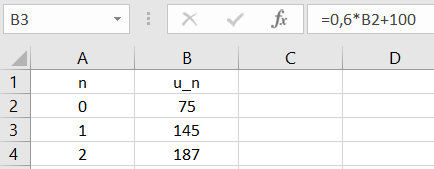
\includegraphics[scale=0.45]{td02_excel_a}
			
			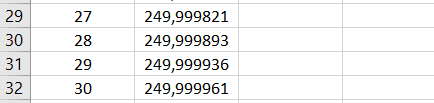
\includegraphics[scale=0.45]{td02_excel_b}
		\end{center}
		\item Les \csheet{valeurs} et \csheet{formules} nécessaires sont \csheet{\helvbx 75} en \csheet{\helvbx B2} ; et \csheet{\helvbx =0,6*B2+100} en \csheet{\helvbx B3}
	\end{enumerate}
	\item On peut conjecturer que le nombre d'abonnés augmente au fil des mois, et stagne vers 250 à long terme.
	\item Le youtubeur va dépasser 230 abonnés au bout de 5 mois car le tableur donne :
	\begin{itemize}
		\item \csheet{\helvbx 227,32} en \csheet{\helvbx B6} soit $u_4 = 227,32 < 230$ ;
		\item \csheet{\helvbx 236,392} en \csheet{\helvbx B7} soit $u_5 = 236,392 > 230$.
	\end{itemize}
%	\begin{center}
%		\includegraphics[scale=0.5]{td01_excel_c}
%	\end{center}
\end{enumerate}
\end{cmanip}

\begin{cmanip}[ - Graphiquement]
\vspace{-0.45cm}
\begin{enumerate}
	\item La fonction $f$ telle que $u_{n+1}=f(u_n)$ est directement $f(x)=0,6x+100$.
	\item On utilise la technique de la \og toile \fg{} en partant -- sur les abscisses -- de $u_0=75$ :
	\begin{center}
		\tunits{0.05}{0.02}
		\tdefgrille{0}{260}{20}{10}{0}{275}{25}{25}
		\begin{tikzpicture}[x=\xunit cm,y=\yunit cm,scale=0.9]
			%AXES & GRILLES
			\tgrilles[line width=0.2pt,lightgray] ;
			\axestikz ;
			\axextikz{0,20,...,240} ;
			\axeytikz{0,25,...,250} ;
			%COURBES
			\draw[line width=1.25pt,red,domain=0:260,samples=260] plot (\x,{\x}) ;
			\draw[line width=1.25pt,blue,domain=0:260,samples=260] plot (\x,{0.6*\x+100}) ;
			%LABELS
			\draw (230,200) node[above right] {\red \large $\Delta$ : $y=x$} ;
			%WEB
			\draw[arrowinside={0.5}{1},line width=1.25pt,purple] (75,0) -- (75,145);
			\draw[arrowinside={0.5}{1},line width=1.25pt,purple] (75,145) -- (145,145);
			\draw[arrowinside={0.5}{1},line width=1.25pt,purple] (145,145) -- (145,187);
			\draw[arrowinside={0.5}{1},line width=1.25pt,purple] (145,187) -- (187,187);
			\draw[arrowinside={0.5}{1},line width=1.25pt,purple] (187,187) -- (187,212.2);
			\draw[arrowinside={0.5}{1},line width=1.25pt,purple] (187,212.2) -- (212.2,212.2);
			\draw[arrowinside={0.5}{1},line width=1.25pt,purple] (212.2,212.2) -- (212.2,227.32);
			\draw[arrowinside={0.5}{1},line width=1.25pt,purple] (212.2,227.32) -- (227.32,227.32);
			\draw[arrowinside={0.5}{1},line width=1.25pt,purple] (227.32,227.32) -- (227.32,236.392);
			\draw[arrowinside={0.5}{1},line width=1.25pt,purple] (227.32,236.392) -- (236.392,236.92);
		\end{tikzpicture}
	\end{center}
%	\begin{center}
%		\psset{xunit=0.05cm,yunit=0.02cm,tickwidth=1pt,algebraic=true}
%		\defgrille{0}{260}{20}{10}{0}{275}{25}{25}
%		\begin{pspicture}(-10,-10)(260,275)
%			\grilles{linewidth=0.2pt,linecolor=lightgray}
%			\psaxes[linewidth=1.25pt,Dx=20,Dy=25]{->}(0,0)(260,275)
%			\psplot[linewidth=1.25pt,linecolor=red]{0}{260}{x}
%			\psplot[linewidth=1.25pt,linecolor=blue]{0}{260}{0.6*x+100}
%			\uput[ur](230,200){\red \large $\Delta$ : $y=x$}
%			\psline[linewidth=1.25pt,linecolor=purple,ArrowInside=->,ArrowInsidePos=0.5](75,0)(75,145)(145,145)(145,187)(187,187)(187,212.2)(212.2,212.2)(212.2,227.32)(227.32,227.32)(227.32,236.392)(236.392,236.92)
%		\end{pspicture}
%	\end{center}
	\item L'\og escalier \fg{} obtenu permet de retrouver le fait que la suite $\suiten$ est croissante (\og vers la droite \fg) et convergente vers 250 (\og point fixe \fg).
\end{enumerate}
\end{cmanip}

\begin{cmanip}[ - Par algorithme]
\vspace{-0.45cm}
\begin{enumerate}
	\item 
	\begin{enumerate}
		\item L'algoithme (classique) de calcul de termes d'une suite récurrente est : \vspace{-0.05cm}
\begin{tcpseudocode}[15cm]
Algorithme : CALCUL DU TERME D'INDICE n
Variables : u == réel ; n == entier ; i == entier
Début
	Afficher("Saisir l'indice n : ")
	Saisir(n)
	u = 75                              #terme initial
	Pour i allant de 1 à n Faire        #répétition n fois (pour u_n)
		u = 0.6 * u + 100               #formule de récurrence
	FinPour
	Afficher(u)                         #affichage de u_n
Fin
\end{tcpseudocode}
		\item En \calgpython{}, la transcription est simple, en faisant attention au \cpy{range} : 
		
		\begin{center}
			\begin{minipage}{0.45\linewidth}
				\begin{envpython}[7.5cm]
					#version classique
					n = int(input("Saisir l'indice n : "))
					u = 75
					for i in range(1,n+1):
						u = 0.6 * u + 100
					print(u)
				\end{envpython}
			\end{minipage}
			\hfill~
			\begin{minipage}{0.45\linewidth}
				\begin{envpython}[7.5cm]
					#version fonctionnelle
					def terme_un(n):
						u = 75
						for i in range(1,n+1):
							u = 0.6 * u + 100
						return u
				\end{envpython}
			\end{minipage}
		\end{center}
	\end{enumerate}
	\item
	\begin{enumerate}
		\item Il s'agit d'un classique algorithme de seuil : \vspace{-0.25cm}
\begin{tcpseudocode}[15cm]
Algorithme : SEUIL 230
Variables : u == réel ; n == entier
Début
	n = 0                           #initialisation de n
	u = 75                          #terme initial de u_n
	TantQue u < 230 Faire           #condition
		u = 0.6*u + 100             #formule de récurrence
		n = n + 1                   #on augmente le compteur
	FinTantQue
	Afficher(n,u)                   #on affiche le rang et le seuil dépassé
Fin
\end{tcpseudocode}	
	\item En \calgpython{}, on obtient :
	
	\begin{center}
		\begin{minipage}{0.45\linewidth}
			\begin{envpython}[7.5cm]
				#version classique
				n = 0
				u = 75
				while u < 230 :
					n = n+1
					u = 0.6 * u + 100
				print(n,u)
			\end{envpython}
		\end{minipage}
		\hfill~
		\begin{minipage}{0.45\linewidth}
			\begin{envpython}[7.5cm]
				def seuil():
					n = 0
					u = 75
					while u < 230 :
						u = 0.6 * u + 100
						n = n+1
					return n,u
			\end{envpython}
		\end{minipage}
	\end{center}
	
	Il suffit d'appeler la fonction \cpy{seuil()} pour retrouver le résultat \og lu \fg{} sur le tableur :
	\begin{consolepython}[15cm]
		\begin{pyconsole}[][framesep=3mm,frame=single,label={[\scriptsize Début de la console \logopython]\scriptsize Fin de la console \logopython},fontsize=\footnotesize,framerule=1pt,rulecolor=\color{ForestGreen}]
			seuil()
		\end{pyconsole}
	\end{consolepython}
	\end{enumerate}
\end{enumerate}
\end{cmanip}

\end{document}